\stepcounter{section}
\begin{center}
	\textbf{\color{color2}\LARGE \thesection} \quad  \textbf{\LARGE Situación nutricional de la madre} \addcontentsline{toc}{section}{\numberline{\thesection} Situación nutricional de la madre}
\end{center}
$ \ $ \\[-5cm]%#########################1########################

 \cajita{%
Mujeres con anemia }%
{Para el año 2008 se registró que del total de las madres embarazadas el 29.1\% padecía anemia, mientras que en las mujeres que no se encontraban en gestación el porcentaje de anemia bajó en 7.7 puntos porcentuales. 
 }%
{%
 Mujeres con anemia, según estado de gestación} %
{%
 República de Guatemala, 2008-2009, en porcentaje} %
{%
 \begin{tikzpicture}[x=1pt,y=1pt]  \input{graficas/6_01.tex}  \end{tikzpicture}}%
{%
Encuesta Nacional de Salud Materno Infantil (Ensmi), 2008/2009 } %

%#########################2########################

\cajita{%
	Índice de Masa Corporal (IMC) de mujeres  }%
{%
	La mayoría de las mujeres guatemaltecas que no se encontraban embarazadas en el 2008 presentaba un IMC normal, mientras que solo un 1.6\% tenía IMC bajo. 
}%
{%
	Índice de masa corporal de mujeres no embarazadas} %
{%
	República de Guatemala, 2008-2009, en porcentaje} %
{%
	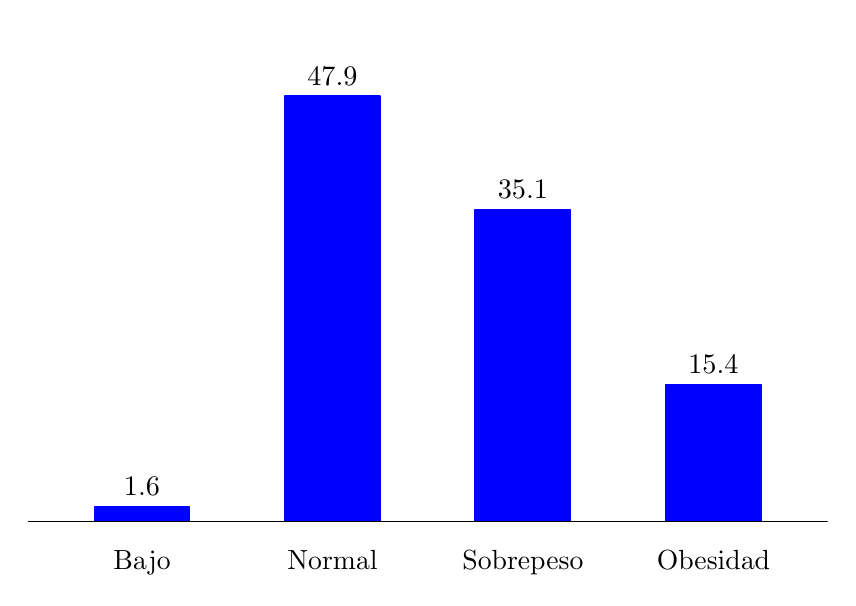
\begin{tikzpicture}[x=1pt,y=1pt]  % Created by tikzDevice version 0.9 on 2016-03-03 06:06:28
% !TEX encoding = UTF-8 Unicode
\definecolor{fillColor}{RGB}{255,255,255}
\path[use as bounding box,fill=fillColor,fill opacity=0.00] (0,0) rectangle (289.08,198.74);
\begin{scope}
\path[clip] (  0.00,  0.00) rectangle (289.08,198.74);

\path[] (  0.00,  0.00) rectangle (289.08,198.74);
\end{scope}
\begin{scope}
\path[clip] (  0.00,  0.00) rectangle (289.08,198.74);

\path[] (  0.00, 12.77) rectangle (289.08,181.67);

\path[] ( 41.30, 12.77) --
	( 41.30,181.67);

\path[] (110.13, 12.77) --
	(110.13,181.67);

\path[] (178.95, 12.77) --
	(178.95,181.67);

\path[] (247.78, 12.77) --
	(247.78,181.67);
\definecolor{drawColor}{RGB}{0,0,255}
\definecolor{fillColor}{RGB}{0,0,255}

\path[draw=drawColor,line width= 0.6pt,line join=round,fill=fillColor] ( 24.09, 20.44) rectangle ( 58.50, 25.57);

\path[draw=drawColor,line width= 0.6pt,line join=round,fill=fillColor] ( 92.92, 20.44) rectangle (127.33,173.99);

\path[draw=drawColor,line width= 0.6pt,line join=round,fill=fillColor] (161.75, 20.44) rectangle (196.16,132.96);

\path[draw=drawColor,line width= 0.6pt,line join=round,fill=fillColor] (230.58, 20.44) rectangle (264.99, 69.81);
\definecolor{drawColor}{RGB}{0,0,0}

\path[draw=drawColor,line width= 0.1pt,line join=round] (  0.00, 20.44) -- (289.08, 20.44);

\node[text=drawColor,anchor=base,inner sep=0pt, outer sep=0pt, scale=  1.02] at ( 41.30, 29.54) {1.6};

\node[text=drawColor,anchor=base,inner sep=0pt, outer sep=0pt, scale=  1.02] at (110.13,177.96) {47.9};

\node[text=drawColor,anchor=base,inner sep=0pt, outer sep=0pt, scale=  1.02] at (178.95,136.93) {35.1};

\node[text=drawColor,anchor=base,inner sep=0pt, outer sep=0pt, scale=  1.02] at (247.78, 73.78) {15.4};

\path[] (  0.00, 12.77) rectangle (289.08,181.67);
\end{scope}
\begin{scope}
\path[clip] (  0.00,  0.00) rectangle (289.08,198.74);

\path[] (  0.00, 12.77) --
	(289.08, 12.77);
\end{scope}
\begin{scope}
\path[clip] (  0.00,  0.00) rectangle (289.08,198.74);

\path[] ( 41.30, 10.02) --
	( 41.30, 12.77);

\path[] (110.13, 10.02) --
	(110.13, 12.77);

\path[] (178.95, 10.02) --
	(178.95, 12.77);

\path[] (247.78, 10.02) --
	(247.78, 12.77);
\end{scope}
\begin{scope}
\path[clip] (  0.00,  0.00) rectangle (289.08,198.74);
\definecolor{drawColor}{RGB}{0,0,0}

\node[text=drawColor,anchor=base,inner sep=0pt, outer sep=0pt, scale=  1.00] at ( 41.30, 3.00) {Bajo};

\node[text=drawColor,anchor=base,inner sep=0pt, outer sep=0pt, scale=  1.00] at (110.13, 3.00) {Normal};

\node[text=drawColor,anchor=base,inner sep=0pt, outer sep=0pt, scale=  1.00] at (178.95, 3.00) {Sobrepeso};

\node[text=drawColor,anchor=base,inner sep=0pt, outer sep=0pt, scale=  1.00] at (247.78, 3.00) {Obesidad};
\end{scope}
  \end{tikzpicture}}%
{%
	Encuesta Nacional de Salud Materno Infantil (Ensmi), 2008/2009} %


%#########################3########################

\cajita{%
	IMC de mujeres, según área de residencia }%
{%
	En el área urbana se presenta mayor proporción de mujeres con sobrepeso y obesidad (37.5\% y 20.3\%) que en el área rural (33.4\% y 12.1\%). 
	Además, el área rural presenta mayor proporción de mujeres con IMC normal que el área urbana. 
}%
{%
	Índice de Masa Corporal (IMC) de mujeres no embarazadas, según área de residencia} %
{%
	República de Guatemala, 2008-2009, en porcentaje} %
{%
	\begin{tikzpicture}[x=1pt,y=1pt]  % Created by tikzDevice version 0.9 on 2016-03-03 06:06:32
% !TEX encoding = UTF-8 Unicode
\definecolor{fillColor}{RGB}{255,255,255}
\path[use as bounding box,fill=fillColor,fill opacity=0.00] (0,0) rectangle (289.08,198.74);
\begin{scope}
\path[clip] (  0.00,  0.00) rectangle (289.08,198.74);

\path[] (  0.00,  0.00) rectangle (289.08,198.74);
\end{scope}
\begin{scope}
\path[clip] (  0.00,  0.00) rectangle (289.08,198.74);

\path[] (  0.00, 18.46) rectangle (289.08,166.57);

\path[] ( 41.30, 18.46) --
	( 41.30,166.57);

\path[] (110.13, 18.46) --
	(110.13,166.57);

\path[] (178.95, 18.46) --
	(178.95,166.57);

\path[] (247.78, 18.46) --
	(247.78,166.57);
\definecolor{drawColor}{RGB}{0,0,255}
\definecolor{fillColor}{RGB}{0,0,255}

\path[draw=drawColor,line width= 0.6pt,line join=round,fill=fillColor] ( 12.05, 18.46) rectangle ( 39.58, 23.49);
\definecolor{drawColor}{RGB}{157,187,255}
\definecolor{fillColor}{RGB}{157,187,255}

\path[draw=drawColor,line width= 0.6pt,line join=round,fill=fillColor] ( 43.02, 18.46) rectangle ( 70.55, 22.65);
\definecolor{drawColor}{RGB}{0,0,255}
\definecolor{fillColor}{RGB}{0,0,255}

\path[draw=drawColor,line width= 0.6pt,line join=round,fill=fillColor] ( 80.87, 18.46) rectangle (108.40,131.64);
\definecolor{drawColor}{RGB}{157,187,255}
\definecolor{fillColor}{RGB}{157,187,255}

\path[draw=drawColor,line width= 0.6pt,line join=round,fill=fillColor] (111.85, 18.46) rectangle (139.38,166.57);
\definecolor{drawColor}{RGB}{0,0,255}
\definecolor{fillColor}{RGB}{0,0,255}

\path[draw=drawColor,line width= 0.6pt,line join=round,fill=fillColor] (149.70, 18.46) rectangle (177.23,123.26);
\definecolor{drawColor}{RGB}{157,187,255}
\definecolor{fillColor}{RGB}{157,187,255}

\path[draw=drawColor,line width= 0.6pt,line join=round,fill=fillColor] (180.68, 18.46) rectangle (208.21,111.80);
\definecolor{drawColor}{RGB}{0,0,255}
\definecolor{fillColor}{RGB}{0,0,255}

\path[draw=drawColor,line width= 0.6pt,line join=round,fill=fillColor] (218.53, 18.46) rectangle (246.06, 75.19);
\definecolor{drawColor}{RGB}{157,187,255}
\definecolor{fillColor}{RGB}{157,187,255}

\path[draw=drawColor,line width= 0.6pt,line join=round,fill=fillColor] (249.50, 18.46) rectangle (277.03, 52.27);
\definecolor{drawColor}{RGB}{0,0,0}

\path[draw=drawColor,line width= 0.6pt,line join=round] (  0.00, 18.46) -- (289.08, 18.46);

\node[text=drawColor,anchor=base west,inner sep=0pt, outer sep=0pt, scale=  0.83] at ( 23.05, 25.31) {1.8};

\node[text=drawColor,anchor=base west,inner sep=0pt, outer sep=0pt, scale=  0.83] at ( 54.02, 24.47) {1.5};

\node[text=drawColor,anchor=base west,inner sep=0pt, outer sep=0pt, scale=  0.83] at ( 91.87,134.19) {40.5};

\node[text=drawColor,anchor=base west,inner sep=0pt, outer sep=0pt, scale=  0.83] at (122.85,169.12) {53.0};

\node[text=drawColor,anchor=base west,inner sep=0pt, outer sep=0pt, scale=  0.83] at (160.70,125.81) {37.5};

\node[text=drawColor,anchor=base west,inner sep=0pt, outer sep=0pt, scale=  0.83] at (191.68,114.35) {33.4};

\node[text=drawColor,anchor=base west,inner sep=0pt, outer sep=0pt, scale=  0.83] at (229.53, 77.74) {20.3};

\node[text=drawColor,anchor=base west,inner sep=0pt, outer sep=0pt, scale=  0.83] at (260.50, 54.82) {12.1};

\path[] (  0.00, 18.46) rectangle (289.08,166.57);
\end{scope}
\begin{scope}
\path[clip] (  0.00,  0.00) rectangle (289.08,198.74);

\path[] (  0.00, 18.46) --
	(289.08, 18.46);
\end{scope}
\begin{scope}
\path[clip] (  0.00,  0.00) rectangle (289.08,198.74);

\path[] ( 41.30, 15.71) --
	( 41.30, 18.46);

\path[] (110.13, 15.71) --
	(110.13, 18.46);

\path[] (178.95, 15.71) --
	(178.95, 18.46);

\path[] (247.78, 15.71) --
	(247.78, 18.46);
\end{scope}
\begin{scope}
\path[clip] (  0.00,  0.00) rectangle (289.08,198.74);
\definecolor{drawColor}{RGB}{0,0,0}

\node[text=drawColor,anchor=base,inner sep=0pt, outer sep=0pt, scale=  1.00] at ( 41.30,  5.69) {Bajo};

\node[text=drawColor,anchor=base,inner sep=0pt, outer sep=0pt, scale=  1.00] at (110.13,  5.69) {Normal};

\node[text=drawColor,anchor=base,inner sep=0pt, outer sep=0pt, scale=  1.00] at (178.95,  5.69) {Sobre peso};

\node[text=drawColor,anchor=base,inner sep=0pt, outer sep=0pt, scale=  1.00] at (247.78,  5.69) {Obesidad};
\end{scope}
\begin{scope}
\path[clip] (  0.00,  0.00) rectangle (289.08,198.74);
\coordinate (apoyo) at (57.27,191.13);
\coordinate (longitudFicticia) at (7.11,7.61);
\coordinate (longitud) at (7.11,7.11);
\coordinate (desX) at (142.24,0);
\coordinate (desY) at (0,0.25);
\definecolor[named]{ct1}{HTML}{
0000FF
}
\definecolor[named]{ct2}{HTML}{
9DBBFF
}
\definecolor[named]{ctb1}{HTML}{
0000FF
}
\definecolor[named]{ctb2}{HTML}{
9DBBFF
}
\path [fill=none] (apoyo) rectangle ($(apoyo)+(longitudFicticia)$)
node [xshift=0.3cm,inner sep=0pt, outer sep=0pt,midway,right,scale = 0.9]{Urbana};
\draw [color = ctb1,fill=ct1] ( $(apoyo)  + (desY) $) rectangle ($(apoyo)+ (desY) +(longitud)$);
\path [fill=none] ($(apoyo)+(desX)$) rectangle ($(apoyo)+(desX)+(longitudFicticia)$)
node [xshift=0.3cm,inner sep=0pt, outer sep=0pt,midway,right,scale = 0.9]{Rural};
\draw [color = ctb2 ,fill=ct2] ( $(apoyo)  + (desY) + (desX) $) rectangle ($(apoyo)+ (desY)+ (desX) +(longitud)$);
\end{scope}
  \end{tikzpicture}}%
{%
	Encuesta Nacional de Salud Materno Infantil (Ensmi), 2008/2009} %


%#########################4########################

\cajita{%
	Talla promedio según área de residencia }%
{%
	Para el 2008 la talla\footnote{Hace referencia a la estatura de una persona, y en este caso se presenta en centímetros.} para madres del área urbana de niños menores de 5 años es apenas mayor que la de las madres del área rural. 
}%
{%
	Talla promedio de madres  de niños menores de 5 años, según área de residencia} %
{%
	República de Guatemala, 2008-2009, en centímetros} %
{%
	\begin{tikzpicture}[x=1pt,y=1pt]  \input{graficas/6_04.tex}  \end{tikzpicture}}%
{%
	Encuesta Nacional de Salud Materno Infantil (Ensmi), 2008/2009} %

%#########################5########################
\stepcounter{section}
\begin{center}
	\textbf{\color{color2}\LARGE \thesection} \quad  \textbf{\LARGE Situación nutricional del niño} \addcontentsline{toc}{section}{\numberline{\thesection} Situación nutricional del niño}
\end{center} $ \ $\\[-5cm]
\cajita{%
	Peso de niños recién nacidos }%
{%
	Uno de los datos más importantes que debe ser medido en un neonato es el peso.
	Para el 2008, el 88.1\% de los recién nacidos presentó un peso no menor de  2.5 kilogramos. 
}%
{%
	Distribución de niños recién nacidos, según peso (en kilogramos), reportado por la madre} %
{%
	República de Guatemala, 2008-2009, en porcentaje} %
{%
	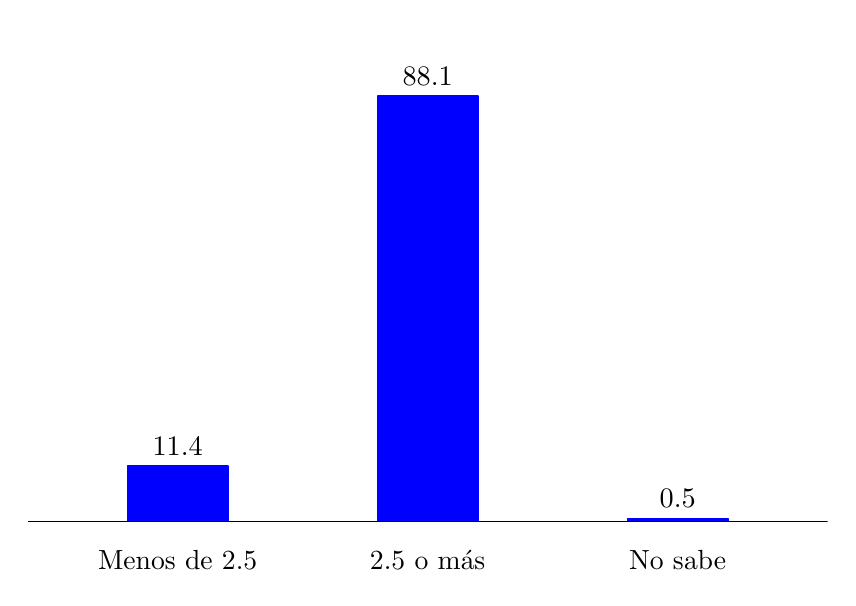
\begin{tikzpicture}[x=1pt,y=1pt]  % Created by tikzDevice version 0.9 on 2016-03-03 06:06:40
% !TEX encoding = UTF-8 Unicode
\definecolor{fillColor}{RGB}{255,255,255}
\path[use as bounding box,fill=fillColor,fill opacity=0.00] (0,0) rectangle (289.08,198.74);
\begin{scope}
\path[clip] (  0.00,  0.00) rectangle (289.08,198.74);

\path[] (  0.00,  0.00) rectangle (289.08,198.74);
\end{scope}
\begin{scope}
\path[clip] (  0.00,  0.00) rectangle (289.08,198.74);

\path[] (  0.00, 12.77) rectangle (289.08,181.67);

\path[] ( 54.20, 12.77) --
	( 54.20,181.67);

\path[] (144.54, 12.77) --
	(144.54,181.67);

\path[] (234.88, 12.77) --
	(234.88,181.67);
\definecolor{drawColor}{RGB}{0,0,255}
\definecolor{fillColor}{RGB}{0,0,255}

\path[draw=drawColor,line width= 0.6pt,line join=round,fill=fillColor] ( 36.13, 20.44) rectangle ( 72.27, 40.31);

\path[draw=drawColor,line width= 0.6pt,line join=round,fill=fillColor] (126.47, 20.44) rectangle (162.61,173.99);

\path[draw=drawColor,line width= 0.6pt,line join=round,fill=fillColor] (216.81, 20.44) rectangle (252.95, 21.32);
\definecolor{drawColor}{RGB}{0,0,0}

\path[draw=drawColor,line width= 0.1pt,line join=round] (  0.00, 20.44) -- (289.08, 20.44);

\node[text=drawColor,anchor=base,inner sep=0pt, outer sep=0pt, scale=  1.02] at ( 54.20, 44.28) {11.4};

\node[text=drawColor,anchor=base,inner sep=0pt, outer sep=0pt, scale=  1.02] at (144.54,177.96) {88.1};

\node[text=drawColor,anchor=base,inner sep=0pt, outer sep=0pt, scale=  1.02] at (234.88, 25.29) {0.5};

\path[] (  0.00, 12.77) rectangle (289.08,181.67);
\end{scope}
\begin{scope}
\path[clip] (  0.00,  0.00) rectangle (289.08,198.74);

\path[] (  0.00, 12.77) --
	(289.08, 12.77);
\end{scope}
\begin{scope}
\path[clip] (  0.00,  0.00) rectangle (289.08,198.74);

\path[] ( 54.20, 10.02) --
	( 54.20, 12.77);

\path[] (144.54, 10.02) --
	(144.54, 12.77);

\path[] (234.88, 10.02) --
	(234.88, 12.77);
\end{scope}
\begin{scope}
\path[clip] (  0.00,  0.00) rectangle (289.08,198.74);
\definecolor{drawColor}{RGB}{0,0,0}

\node[text=drawColor,anchor=base,inner sep=0pt, outer sep=0pt, scale=  1.00] at ( 54.20, 3.00) {Menos de 2.5 };

\node[text=drawColor,anchor=base,inner sep=0pt, outer sep=0pt, scale=  1.00] at (144.54, 3.00) {2.5  o más};

\node[text=drawColor,anchor=base,inner sep=0pt, outer sep=0pt, scale=  1.00] at (234.88, 3.00) {No sabe};
\end{scope}
  \end{tikzpicture}}%
{%
	Encuesta Nacional de Salud Materno Infantil (Ensmi), 2008/2009} %

%#########################6########################

\cajita{%
	Desnutrición global }%
{%
	La tasa de desnutricion global total para el 2008 fue de 13.1\%, siendo el 2.1\% desnutrición global severa. 
}%
{%
	Niños menores de 5 años con desnutrición global} %
{%
	República de Guatemala, 2008-2009, en porcentaje} %
{%
	\begin{tikzpicture}[x=1pt,y=1pt]  \input{graficas/6_05.tex}  \end{tikzpicture}}%
{%
	Encuesta Nacional de Salud Materno Infantil (Ensmi), 2008/2009} %

%#########################7########################

\cajita{%
	Desnutrición aguda }%
{%
	La desnutrición aguda (bajo peso para la talla) se ubicó en 1.4\% para el 2008.
}%
{%
	Niños menores de 5 años con desnutrición aguda} %
{%
	República de Guatemala, 2008-2009, en porcentaje} %
{%
	\begin{tikzpicture}[x=1pt,y=1pt]  \input{graficas/6_06.tex}  \end{tikzpicture}}%
{%
	Encuesta Nacional de Salud Materno Infantil (Ensmi), 2008/2009} %


%#########################8########################

\cajita{%
	Desnutrición crónica }%
{%
	La desnutrición crónica es el retraso del crecimiento esperado para una edad. 
	
	Para niños menores de 5 años se observó en 2008 que el 49.8\% de estos presenta una talla menor a la esperada para su edad, es decir que se encontraban con desnutrición crónica. 
}%
{%
	Niños menores de 5 años con desnutrición crónica} %
{%
	República de Guatemala, 2008-2009, en porcentaje} %
{%
	\begin{tikzpicture}[x=1pt,y=1pt]  \input{graficas/6_07.tex}  \end{tikzpicture}}%
{%
	Encuesta Nacional de Salud Materno Infantil (Ensmi), 2008/2009} %


%#########################9########################

\cajita{%
	Niños con anemia }%
{%
	El área rural presenta mayor porcentaje de niños con anemia, ubicándose en 48.6\%, esto está 2.4 puntos por arriba del indicador para el área urbana. 
	}%
{%
	Niños entre 6 y 59 meses con anemia, según área de residencia} %
{%
	República de Guatemala, 2008-2009, en porcentaje} %
{%
	\begin{tikzpicture}[x=1pt,y=1pt]  \input{graficas/6_08.tex}  \end{tikzpicture}}%
{%
	Encuesta Nacional de Salud Materno Infantil (Ensmi), 2008/2009} %

%#########################9########################

\cajota{%
	Niños con anemia por departamento }%
{%
	El departamento de Suchitepéquez es el que presenta menor porcentaje de niños con anemia (37.7\%), seguido de El Progreso (37.8\%), y Quetzaltenango (40.2\%). Los departamentos con mayor porcentaje de anemia en niños son Totonicapán (62.2\%), Sololá (56.1\%), y Chiquimula (55.5\%).
}%
{%
	Niños entre 6 y 59 meses con anemia por departamento} %
{%
	República de Guatemala, 2008-2009, en porcentaje} %
{%
	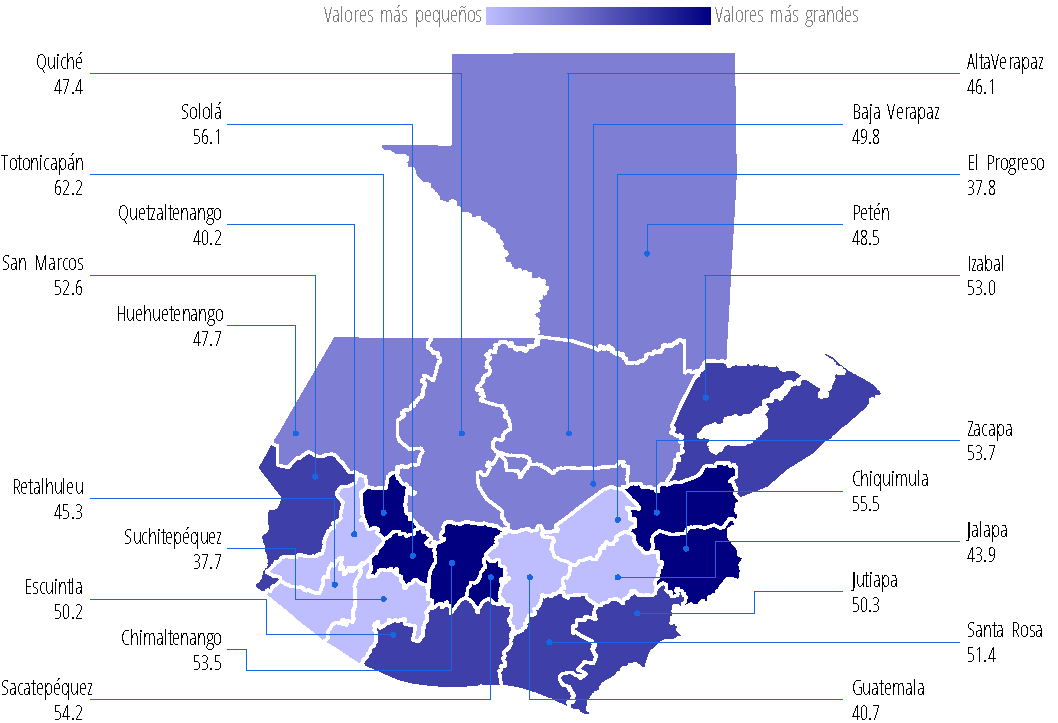
\includegraphics[width=52\cuadri]{graficas/6_09.pdf}}%
{%
	Encuesta Nacional de Salud Materno Infantil (Ensmi), 2008/2009} %